\documentclass[12pt, a4paper, oneside]{article}
\usepackage{ctex}
\usepackage{amsmath, amsthm, amssymb, appendix, bm, graphicx, hyperref, mathrsfs}
% 设置页边距
\usepackage{geometry}
\geometry{left=2.5cm,right=2.5cm,top=2.54cm,bottom=2.54cm}
% 使用图片包
\usepackage{graphicx}
\usepackage{caption}
% 动画宏包
\usepackage[scale=0.8]{animate}
% 代码展示
\usepackage{listings} 
\usepackage{color}
\definecolor{dkgreen}{rgb}{0,0.6,0}
\definecolor{gray}{rgb}{0.5,0.5,0.5}
\definecolor{mauve}{rgb}{0.58,0,0.82}
% 超链接
\usepackage{hyperref}


\lstset{ %
	language={[x86masm]Assembler},                % the language of the code
	basicstyle=\ttfamily\footnotesize,           % the size and type of the fonts that are used for the code
	numbers=left,                   % where to put the line-numbers
	numberstyle=\tiny\color{gray},  % the style that is used for the line-numbers
	stepnumber=1,                   % the step between two line-numbers. If it's 1, each line will be numbered
	numbersep=5pt,                  % how far the line-numbers are from the code
	backgroundcolor=\color{white},      % choose the background color. You must add \usepackage{color}
	showspaces=false,               % show spaces adding particular underscores
	showstringspaces=false,         % underline spaces within strings
	showtabs=false,                 % show tabs within strings adding particular underscores
	frame=single,                   % adds a frame around the code
	rulecolor=\color{black},        % if not set, the frame-color may be changed on line-breaks within not-black text (e.g. commens (green here))
	tabsize=2,                      % sets default tabsize to 2 spaces
	captionpos=b,                   % sets the caption-position to bottom
	breaklines=true,                % sets automatic line breaking
	breakatwhitespace=false,        % sets if automatic breaks should only happen at whitespace
	title=\lstname,                   % show the filename of files included with \lstinputlisting; also try caption instead of title
	keywordstyle=\color{blue},          % keyword style
	commentstyle=\color{dkgreen},       % comment style
	stringstyle=\color{mauve},         % string literal style
	escapeinside={\%*}{*)},            % if you want to add LaTeX within your code
	morekeywords={*,...}               % if you want to add more keywords to the set
}

\linespread{1.5}

\title{双摆的动力学模拟与其混沌现象的探究}
\author{10Q22104陈诚}
\date{2024.6.1}

\begin{document}

\maketitle

\begin{abstract}
双摆是一向比较基本的物理学模型,由于其具有一定的混沌行为从而难以解析求解.在本项目中,我们研究了双摆系统,并通过数值模拟计算其Lyapunov指数.我们首先建立了双摆系统的运动方程,使用拉格朗日力学推导出二阶非线性微分方程,并将其转换为一阶方程组.然后,我们编写了C++程序,使用四阶Runge-Kutta方法求解这些方程.为了分析混沌行为,我们引入了微小扰动,通过计算扰动状态与初始状态之间的分离度量,利用求得Lyapunov指数.同时,我们使用MATLAB读取数值模拟数据,并绘制双摆的运动轨迹和角度随时间变化的图,以可视化双摆系统的混沌特性.
\end{abstract}

\section{双摆问题}

\subsection{物理模型}
双摆由两个摆组成,第一个摆长度为$l_1$,质量为$m_1$,第二个摆长度为$l_2$,质量为$m_2$.描述这个系统可以使用拉格朗日力学,取广义坐标为$\left(\theta_1 , \theta_2 \right)$.如图\ref{fig:double_pendulums}所示.
\begin{figure}[htbp]
	\centering
	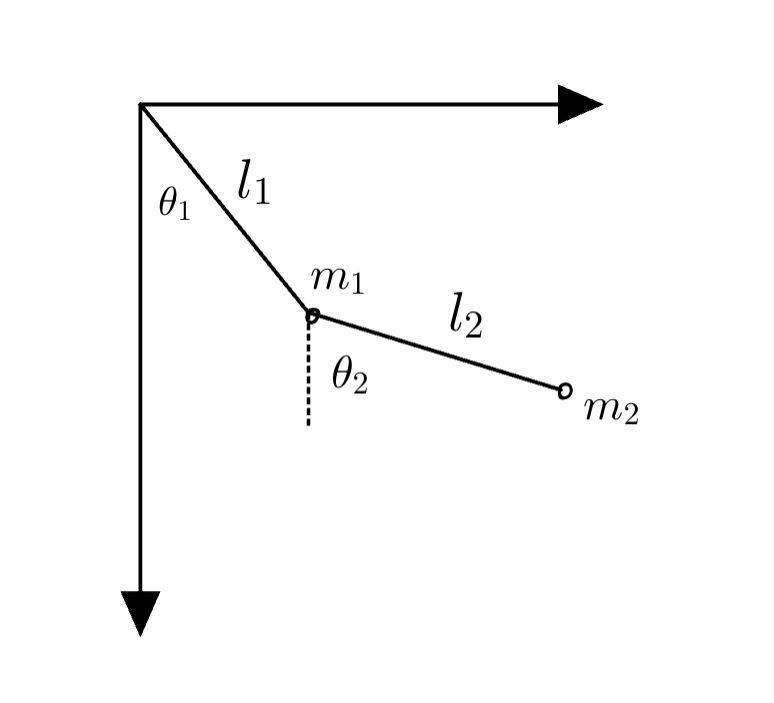
\includegraphics[width = 10 cm]{figures/double_pendulum.jpg}
	\caption{Double pendulums}
	\label{fig:double_pendulums}
\end{figure}
\subsection{拉格朗日力学}
由
\begin{align*}
x_1 &= l_1 \sin\theta_1 &	x_2 &= l_1 \sin\theta_1 + l_2 \sin\theta_2 \\
y_1 &= -l_1 \cos\theta_1 &	y_2 &= -l_1 \cos\theta_1 - l_2 \cos\theta_2
\end{align*}
计算动能$T$和势能$V$:
\begin{align}
	T &= \frac{1}{2} m_1 ( \dot{x}_1^2 + \dot{y}_1^2 ) + \frac{1}{2} m_2 ( \dot{x}_2^2 + \dot{y}_2^2 ) \notag \\
	& = \frac{1}{2} m_1 \left(\dot{l_1} \right)^2 + \frac{1}{2} m_2 \left[ ( l_1 \dot{\theta}_1 )^2 + ( l_2 \dot{\theta}_2 )^2 + 2l_1l_2\dot{\theta}_1\dot{\theta}_2\cos(\theta_1 - \theta_2) \right] \\
	V &= m_1gy_1 + m_2gy_2 \notag \\
	& = - m_1gl_1 \cos\theta_1 - m_2g(l_1\cos\theta_1 + l_2\cos\theta_2)
\end{align}
可得拉格朗日量$L$为
\begin{align}
	L &= T -V  \notag \\
	&= \frac{m_1 + m_2}{2} l_1^2 \dot{\theta}_1^2 + \frac{m_2}{2} l_2^2 \dot{\theta}_2^2 + m_2l_1l_2\cos(\theta_1 - \theta_2)\dot{\theta}_1\dot{\theta}_2 \notag \\ 
	&+ (m_1+m_2)gl_1\cos\theta_1 + m_2gl_2\cos\theta_2
\end{align}
动力学过程由拉格朗日方程给出
\begin{equation}
	\frac{\mathrm{d}}{\mathrm{d}t} \frac{\partial L}{\partial \dot{\theta}_i} - \frac{\partial L}{\partial \theta_i} = 0 (i = 1,2)
\end{equation}
通过引入新变量$\omega_1 = \Dot{\theta}_1$,$\omega_2 = \Dot{\theta}_2$,我们将二阶OED转化成一阶OED方程组,通过数值方法求解方程.
\[
\begin{aligned}
\dot{\theta}_1 &= \omega_1, \\
\dot{\omega}_1 &= \frac{m_2 l_1 \omega_1^2 \sin(\theta_2 - \theta_1) \cos(\theta_2 - \theta_1) + m_2 g \sin\theta_2 \cos(\theta_2 - \theta_1) + m_2 l_2 \omega_2^2 \sin(\theta_2 - \theta_1) - (m_1 + m_2) g \sin\theta_1}{(m_1 + m_2) l_1 - m_2 l_1 \cos(\theta_2 - \theta_1)^2}, \\
\dot{\theta}_2 &= \omega_2, \\
\dot{\omega}_2 &= \frac{-m_2 l_2 \omega_2^2 \sin(\theta_2 - \theta_1) \cos(\theta_2 - \theta_1) + (m_1 + m_2) (g \sin\theta_1 \cos(\theta_2 - \theta_1) - l_1 \omega_1^2 \sin(\theta_2 - \theta_1) - g \sin\theta_2)}{(l_2 / l_1) ((m_1 + m_2) l_1 - m_2 l_1 \cos(\theta_2 - \theta_1)^2)}.
\end{aligned}
\]

\subsection{数值求解}
使用四阶Runge-Kutta方法求解上述一阶微分方程组.实现代码如附录double pendulums.cpp所示.

\subsection{模拟结果}
由上述c++程序求得双摆的位置信息,并写入文件后,由Matlab读取并绘制双摆的运动图像.绘制不同初始条件下的模拟结果,如图\ref{fig:simulation_results}.\quad Matlab代码如附录double pendunlum plot.m所示.

\begin{figure}[htbp]
	\centering
	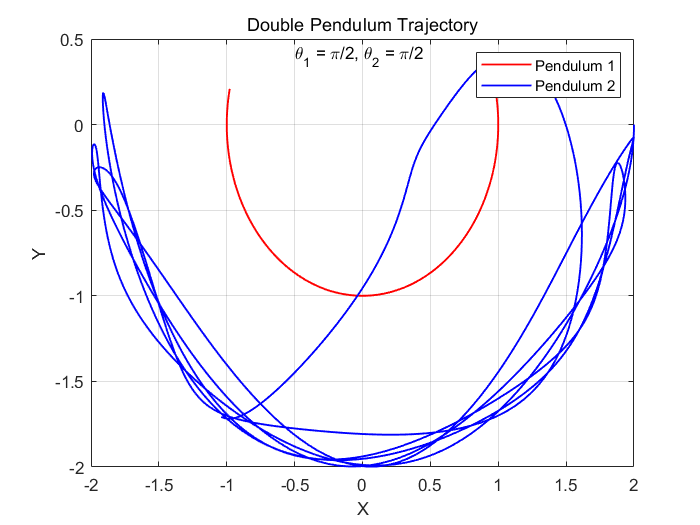
\includegraphics[width = 7cm]{figures/1.png} \qquad
	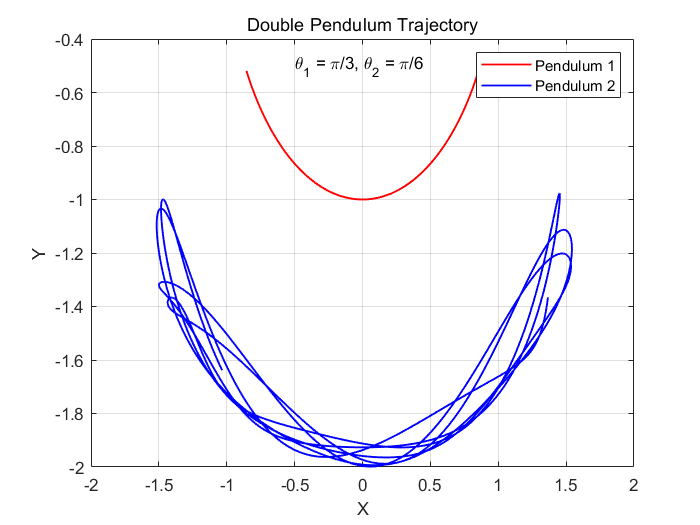
\includegraphics[width = 7cm]{figures/2.png} \\
	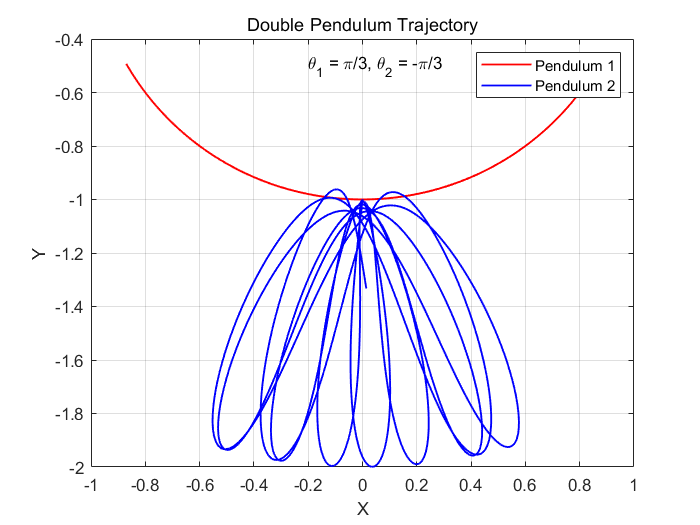
\includegraphics[width = 7cm]{figures/3.png} \qquad
	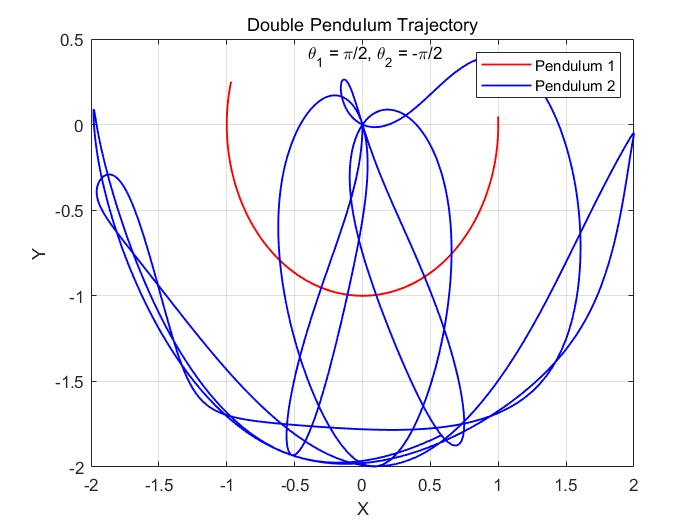
\includegraphics[width = 7cm]{figures/4.png}
	\caption{Simulation results under different initial conditions}
	\label{fig:simulation_results}
\end{figure}

可见双摆的行为对初值敏感,具有明显的混沌特性.下面我们运用Lyapunov指数,来分析这种混沌特性.
\section{Lyapunov分析}
\subsection{Lyapunov指数}
Lyapunov指数是一种用来描述动力系统混沌性质的数学工具.在非线性动力系统中,Lyapunov指数衡量了系统中微小扰动的增长率,从而表征了系统的混沌程度.如果Lyapunov指数为正,这表明微小扰动会指数增长,系统是混沌的;如果Lyapunov指数为负,这表示微小扰动会趋于稳定,系统是非混沌的.Lyapunov指数的正负值以及其大小可以提供关于系统演化行为的重要信息.
\subsection{计算Lyapunov指数}
我们采用最直观的方法计算Lyapunov指数,基于数值模拟数据的线性拟合方法,通过计算两个初始条件非常接近的轨迹随时间的分离情况来确定Lyapunov指数,即:\[\lambda = \lim_{t \to \infty} \frac{1}{t}\log\frac{d(t)}{d(0)}\]其中$d(t)$是时间t时刻的距离,$d(0)$是初始距离.具体步骤如下:
\begin{itemize}
	\item 初始化条件:从一个初始状态开始,并在其基础上施加一个非常小的扰动,得到两个初始状态.
	\item 数值积分:使用数值方法在同样的时间步长下积分两个初始状态,得到它们在每个时间步长上的状态.
	\item 计算分离度量:在每个时间步长上计算两个状态之间的差异.
	\item 取对数:计算分离度量的对数($log$)值.
	\item 线性拟合:将对数分离度量对时间进行线性拟合,拟合斜率即为Lyapunov指数.
\end{itemize}
\subsection{计算Lyapunov指数函数代码}
\begin{lstlisting}[language = C++, name = calculate_lyapunov_exponent]
		double calculate_lyapunov_exponent(double delta_0, const std::vector<double>& times, const std::vector<double>& theta1_1, const std::vector<double>& theta1_2) {
		std::vector<double> log_deltas(times.size());
		for (size_t i = 0; i < times.size(); ++i) {
			double delta_t = std::abs(theta1_1[i] - theta1_2[i]);
			log_deltas[i] = std::log(delta_t / delta_0);
		}

		// 使用线性拟合计算Lyapunov指数
		double sum_t = 0.0, sum_log_delta = 0.0, sum_t_log_delta = 0.0, sum_t2 = 0.0;
		for (size_t i = 0; i < times.size(); ++i) {
			sum_t += times[i];
			sum_log_delta += log_deltas[i];
			sum_t_log_delta += times[i] * log_deltas[i];
			sum_t2 += times[i] * times[i];
		}

		double n = times.size();
		double lyapunov_exponent = (n * sum_t_log_delta - sum_t * sum_log_delta) / (n * sum_t2 - sum_t * sum_t);
		return lyapunov_exponent;
	}
\end{lstlisting}
\subsection{计算Lyapunov指数结果}
通过程序计算,我们可以得到当初始条件$\theta_1 = \pi/2, \theta_2 = \pi/2$时,Lyapunov指数的计算结果为图\ref{fig:lyapunov_exponent}所示.
\begin{figure}[htbp]
	\centering
	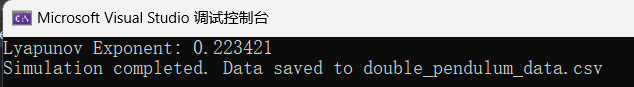
\includegraphics[width = 16 cm]{figures/lyapunov.png}
	\caption{Lyapunov Exponent}
	\label{fig:lyapunov_exponent}
\end{figure}

可见,Lyapunov指数结果为正(0.22),反应双摆系统的混沌效应比较强烈.
\section{总结}
本项目成功实现了双摆系统的数值模拟与混沌行为分析.通过编写C++程序,我们能够准确地求解双摆系统的运动方程,并计算其Lyapunov指数,以定量描述其混沌特性.数值结果表明,双摆系统对初始条件极为敏感,验证了其混沌性质.此外,使用MATLAB进行数据可视化,清晰展示了双摆运动的复杂轨迹和角度随时间的变化.此项目不仅提供了对混沌系统的深刻理解,还展示了数值模拟和数据分析在物理研究中的重要应用.未来的工作可以进一步研究不同参数对双摆系统行为的影响,并探索更复杂的多摆系统的混沌特性.

当然,对于混沌系统,本项目中采用c++编写的Runge-Kutta方法肯定具有一定误差,如果能使用Mathematica或者Matlab等成熟计算软件求解微分方程,该程序无在模拟与计算上都有很多优化的空间,像更复杂的混沌系统拓展也更简易些.

\newpage
\appendix
\section{附录}
\begin{lstlisting}[language = C++, name = double_pendulum_main.cpp]
	#include <iostream>
#include <cmath>
#include <vector>
#include <fstream>
#include <corecrt_math_defines.h>


const double g = 9.81; // 重力加速度

// 双摆系统参数
struct Pendulum {
    double m1, m2; // 质量
    double l1, l2; // 长度
};

// 定义状态向量
struct State {
    double theta1, omega1, theta2, omega2;
};

// 双摆系统的微分方程
std::vector<double> equations(double t, const State& state, const Pendulum& pendulum) {
    double delta_theta = state.theta2 - state.theta1;

    double den1 = (pendulum.m1 + pendulum.m2) * pendulum.l1 - pendulum.m2 * pendulum.l1 * cos(delta_theta) * cos(delta_theta);
    double den2 = (pendulum.l2 / pendulum.l1) * den1;

    double dtheta1_dt = state.omega1;
    double dtheta2_dt = state.omega2;
    double domega1_dt = (pendulum.m2 * pendulum.l1 * state.omega1 * state.omega1 * sin(delta_theta) * cos(delta_theta) +
        pendulum.m2 * g * sin(state.theta2) * cos(delta_theta) +
        pendulum.m2 * pendulum.l2 * state.omega2 * state.omega2 * sin(delta_theta) -
        (pendulum.m1 + pendulum.m2) * g * sin(state.theta1)) / den1;
    double domega2_dt = (-pendulum.m2 * pendulum.l2 * state.omega2 * state.omega2 * sin(delta_theta) * cos(delta_theta) +
        (pendulum.m1 + pendulum.m2) * (g * sin(state.theta1) * cos(delta_theta) -
            pendulum.l1 * state.omega1 * state.omega1 * sin(delta_theta) - g * sin(state.theta2))) / den2;

    return { dtheta1_dt, domega1_dt, dtheta2_dt, domega2_dt };
}

// 四阶Runge-Kutta方法求解器
State runge_kutta_step(double t, const State& state, double dt, const Pendulum& pendulum) {
    auto k1 = equations(t, state, pendulum);
    State state_k2 = { state.theta1 + 0.5 * dt * k1[0], state.omega1 + 0.5 * dt * k1[1],
                       state.theta2 + 0.5 * dt * k1[2], state.omega2 + 0.5 * dt * k1[3] };
    auto k2 = equations(t + 0.5 * dt, state_k2, pendulum);

    State state_k3 = { state.theta1 + 0.5 * dt * k2[0], state.omega1 + 0.5 * dt * k2[1],
                       state.theta2 + 0.5 * dt * k2[2], state.omega2 + 0.5 * dt * k2[3] };
    auto k3 = equations(t + 0.5 * dt, state_k3, pendulum);

    State state_k4 = { state.theta1 + dt * k3[0], state.omega1 + dt * k3[1],
                       state.theta2 + dt * k3[2], state.omega2 + dt * k3[3] };
    auto k4 = equations(t + dt, state_k4, pendulum);

    State new_state;
    new_state.theta1 = state.theta1 + (dt / 6.0) * (k1[0] + 2 * k2[0] + 2 * k3[0] + k4[0]);
    new_state.omega1 = state.omega1 + (dt / 6.0) * (k1[1] + 2 * k2[1] + 2 * k3[1] + k4[1]);
    new_state.theta2 = state.theta2 + (dt / 6.0) * (k1[2] + 2 * k2[2] + 2 * k3[2] + k4[2]);
    new_state.omega2 = state.omega2 + (dt / 6.0) * (k1[3] + 2 * k2[3] + 2 * k3[3] + k4[3]);

    return new_state;
}

double calculate_lyapunov_exponent(double delta_0, const std::vector<double>& times, const std::vector<double>& theta1_1, const std::vector<double>& theta1_2) {
    std::vector<double> log_deltas(times.size());
    for (size_t i = 0; i < times.size(); ++i) {
        double delta_t = std::abs(theta1_1[i] - theta1_2[i]);
        log_deltas[i] = std::log(delta_t / delta_0);
    }

    // 使用线性拟合计算Lyapunov指数
    double sum_t = 0.0, sum_log_delta = 0.0, sum_t_log_delta = 0.0, sum_t2 = 0.0;
    for (size_t i = 0; i < times.size(); ++i) {
        sum_t += times[i];
        sum_log_delta += log_deltas[i];
        sum_t_log_delta += times[i] * log_deltas[i];
        sum_t2 += times[i] * times[i];
    }

    double n = times.size();
    double lyapunov_exponent = (n * sum_t_log_delta - sum_t * sum_log_delta) / (n * sum_t2 - sum_t * sum_t);
    return lyapunov_exponent;
}


int main() {
    // 初始条件////////////修改初始条件在此处/////////////
    State initial_state = { M_PI / 2, 0.0, M_PI / 2, 0.0 };
    State perturbed_state = { M_PI / 2 + 1e-8, 0.0, M_PI / 2, 0.0 };


    // 系统参数
    Pendulum pendulum = { 1.0, 1.0, 1.0, 1.0 };

    // 时间参数
    double t_start = 0.0;
    double t_end = 10.0;
    double dt = 0.01;
    size_t num_steps = static_cast<size_t>((t_end - t_start) / dt);

    // 内存保存时间和状态数据
    std::vector<double> times(num_steps);
    std::vector<double> theta1_1(num_steps), theta1_2(num_steps);
    // 文件保存数据
    std::ofstream file("double_pendulum_data.csv");
    file << "time,theta1,omega1,theta2,omega2\n";

    // 循环求解
    State state = initial_state;
    State perturbed = perturbed_state;
    /*for (double t = t_start; t <= t_end; t += dt) {
        file << t << "," << state.theta1 << "," << state.omega1 << "," << state.theta2 << "," << state.omega2 << "\n";
        state = runge_kutta_step(t, state, dt, pendulum);
    }*/
    for (size_t i = 0; i < num_steps; ++i) {
        double t = t_start + i * dt;
        times[i] = t;
        theta1_1[i] = state.theta1;
        theta1_2[i] = perturbed.theta1;
        file << t << "," << state.theta1 << "," << state.omega1 << "," << state.theta2 << "," << state.omega2 << "\n";
        state = runge_kutta_step(t, state, dt, pendulum);
        perturbed = runge_kutta_step(t, perturbed, dt, pendulum);
    }
   
    
    // 计算Lyapunov指数
        double delta_0 = 1e-8;
    double lyapunov_exponent = calculate_lyapunov_exponent(delta_0, times, theta1_1, theta1_2);
    std::cout << "Lyapunov Exponent: " << lyapunov_exponent << std::endl;


    file.close();
    std::cout << "Simulation completed. Data saved to double_pendulum_data.csv" << std::endl;
    return 0;
}


\end{lstlisting}
\begin{lstlisting}[language = Matlab, name = double pendunlum plot.m]
	data = readtable(['E:\Projects\MSVS\Computational Physics\double pendulum' ...
    '\double pendulum\double_pendulum_data.csv']);

% 提取时间和角度数据
time = data.time;
theta1 = data.theta1;
theta2 = data.theta2;

% 双摆的长度
l1 = 1.0;
l2 = 1.0;

% 绘制角度随时间的变化
% figure;
% plot(time, theta1, 'r', 'DisplayName', '\theta_1');
% hold on;
% plot(time, theta2, 'b', 'DisplayName', '\theta_2');
% xlabel('Time [s]');
% ylabel('Angle [rad]');
% legend;
% title('Double Pendulum Angles');
% grid on;

% 计算双摆末端的坐标
x1 = l1 * sin(theta1);
y1 = -l1 * cos(theta1);
x2 = x1 + l2 * sin(theta2);
y2 = y1 - l2 * cos(theta2);

initconditions = "\theta_1 = \pi/2, \theta_2 = -\pi/2";
% 绘制双摆的运动轨迹
figure;
plot(x1, y1, 'r', 'DisplayName', 'Pendulum 1','LineWidth',1.1);
hold on;
plot(x2, y2, 'b', 'DisplayName', 'Pendulum 2','LineWidth',1.1);
xlabel('X');
ylabel('Y');
legend;
title('Double Pendulum Trajectory');
text(-0.4,0.4,initconditions);
grid on;




\end{lstlisting}


\end{document}